%  Typ dokumentu - článek, prezentace aj.
\documentclass[english]{article}

%  Nastaví vstupní a výstupní kódování znaků (encoding) a lokalizace
%\usepackage[T1]{fontenc}
\usepackage[utf8]{inputenc}
\usepackage[english,czech]{babel}
\usepackage{icomma}
\usepackage{lmodern}

\usepackage{color}
\definecolor{rarek}{rgb}{0.75,0.56,0.00}
\definecolor{kuba}{rgb}{0.60,0.60,0.60}
\definecolor{tonda}{rgb}{0.29,0.53,0.91}
\definecolor{dafit}{rgb}{1.00,0.00,0.00}
\definecolor{pheter}{rgb}{0.00,1.00,0.00}
\definecolor{andras}{rgb}{0.60,0.00,1.00}

%  Formát papíru a odsazení od jeho okrajů
\usepackage[letterpaper]{geometry}
\geometry{verbose,tmargin=1.5cm,bmargin=2cm,lmargin=2cm,rmargin=2cm}

%  Umožňuje pracovat s grafikou
\usepackage{graphicx}
\usepackage{bigstrut}

%  Automaticky odsadí i první paragraf v každé sekci
\usepackage{indentfirst}

\usepackage{enumitem}

%  Umožňuje rozdělovat obsah na více sloupců
\usepackage{multicol}
\usepackage{booktabs}

%  Umožňuje používat hypertextové odkazy, nastavuje jejich barvu a
%  vlastnosti
\usepackage[unicode]{hyperref}
\hypersetup{
colorlinks=true, citecolor=blue, filecolor=blue, linkcolor=blue,
urlcolor=blue
}

%  Umožnění odstranění italiky u jednotek
\newcommand{\unit}[1]{\mathrm{#1}}

%  Formátování stránek, empty = odstraní číslování
% \pagestyle{empty}

%  Řádkování
\linespread{1.2}

%  Lepší zobrazování matematiky (rozšíření sum o \limits atd.)
\everymath{\displaystyle}
\usepackage{amsmath, amsthm, amssymb}

% Umožní psát přes \mathbb{N/R/Q/..} množiny čísel
\usepackage{amssymb}

%  Velikost fontu matematických výrazů v dokumentu lze pro danou
% základního fontu dokumentu upravit pomocí:
% \DeclareMathSizes{X}{Y}{Z}{U} kde:
% X je velikost fontu v dokumentu, pro kterou se matematika upraví
% Y je standartní velikost fontu matematiky
% Z je velikost fontu zmenšených (vnořených výrazů)
% U je velikost fontu ještě více zmenšených (vnořených výrazů).
\DeclareMathSizes{10}{10.5}{9}{9}

%  Nastaví autora, název, datum, skupinu měření apod. (můj vlastní
% příkaz, umožní znovu-použití v dokumentu)
\newcommand{\Author}{Tonda Šnek, daFit $\rho$Esel, András Unoka, Pheter Phvihra, Rarek Most, Jakub Překvapil}
\newcommand{\Coauthor}{Tereza Schönfeldová}
\newcommand{\Institute}{FJFI ČVUT v Praze}
\newcommand{\Subject}{FYZIKÁLNÍ PRAKTIKUM I}
\newcommand{\Group}{7}
\newcommand{\Circle}{ZS 5}
\newcommand{\Title}{Úloha \#0  \\Ukázovký protokol}
\newcommand{\Date}{13.13.2013}

% Začátek dokumentu - Formátování na výstup
\begin{document}

% Interní proměnné, možno zobrazovat u prezentací, používají se při
% generování pomocí \titlepage apod.
\author{\Author}
\title{\Title}
\date{\Date}

%  Lokalizace některých názvů do češtiny
\renewcommand{\figurename}{Obr.}
\renewcommand{\tablename}{Tab.}
\renewcommand{\refname}{Reference}
\renewcommand*\abstractname{Věnování}

% --- Hlavička dokumentu -----------------------------------------------

\setlength{\parindent}{0cm}
\begin{multicols}{2}
\textbf{\Subject \\
        \Institute \\[0.1cm]
%\large  \Title \\[0.5cm]
\Title \\[0.5cm]
}
\begin{tabular}{rl} %l}
\large Datum měření: & \Date \\ %& \large Skupina: & \Group \\
\large Kroužek: & $\circ$ \\ %&\large Klasifikace:\\
\large Klasifikace: & A$^+$ \\
\large Jména: & \Author \\ %& \large Kroužek:  & \Circle\\
\end{tabular}

\begin{flushright}

\includegraphics[scale=0.28]{../../_meta/fjfi_standart.pdf}
\hspace{0.2cm}

\includegraphics[scale=0.28]{../../_meta/cvut_standart.pdf}
\end{flushright}
\end{multicols}
\hrule
\vspace{0.5cm}

% ----------------------------------------------------------------------

% --- Tělo dokumentu ---------------------------------------------------

\begin{abstract}
Váženému kolektivu praktik, aby viděl, že každý protokol “opravdu” trvá 4-6 hodin a že tedy máme spoustu času na dělání protokolů navíc. Tento protokol vznikl jako příspěvek na vánoční besídku EJCF a identity všech asistentů byly kvalitně zašifrovány z důvodu (nejen) jejich bezpečnosti.
\end{abstract}

\setlength{\parindent}{0.5cm}



\section{Pracovní úkoly}
	\begin{enumerate}
		\item Změřte zábavnost praktika metodou totální perspektivy. Naměřená data zpracujte hudebně.
		
		\item Vypočtěte a změřte součinitel opruzu.
		
		\item Úloha pravdy: Změřte co nejvíce věcí v celém praktiku a zpracujte tuto úlohu zcela pravdivě.
		
		\item Změřte a zjistěte následující hodnoty pro jednotlivé asistenty
		\begin{enumerate}[label=\alph*)]
			\item koeficient zábavnosti $Z$,
			\item koeficient čitelnosti hodnocení protokolu $C$,
			\item kvocient přítomnosti u úlohy $P$,
			\item faktor fyzického násilí $N$,
			\item součinitel celkové jednotnosti oprav $O$,
			\item faktor výslechu $V$.
		\end{enumerate}
	\end{enumerate}

\section{Vypracování}
\subsection{Použité přístroje}
Divný stroj co neznáme, odhadové měřítko, další divný stroj co neznáme, něco tak starého, že to snad ani nemůže fungovat, osciloskop, kterému nerozumí ani asistenti, superpočítač s 10 čipy Intel 4004, notebook s připraveným excelem co na místě udělá výpočet finální hodnoty, tři prsteny elfů značky $CELEBRIMBOR$, vír totální perspektivy, rotační senzor $BOMBUR$, program na výrobu grafů $FUUplot$.
\subsection{Teoretický úvod}
\subsubsection{Měření zábavnosti praktika metodou totální perspektivy}
Vír totální perspektivy vynalezl Trin Trangula, aby dokázal, že zkoumání kusů piškotových dortů a přemítání o principu zavíracích špendlíků, má smysl. Na jeden konec stroje připojil veškerou realitu, extrapolovanou z kusu piškotového dortu, a na druhý konec svou ženu. Ta se poté, co jí stroj ukázal veškerou realitu, zbláznila. Podobně také my připojíme na vír totální perspektivy (jak se s ním pracuje, jsme si našli v návodu k přístrojům \cite{bib:pristroje}) data získané z našich měření a extrapolujeme je jako veškerou realitu. Na druhý konec potom připojíme notebook s připraveným excelem a doufáme, že se, na rozdíl od ženy Trina Tranguli, nezblázní. Zábavnost praktik následně určíme z koeficientu $Z$, který nám excel vypočítá na základě totální perspektivy.  
\subsubsection{Součinitel opruzu}
Součinitel opruzu $O$ byl objeven současně se zábavností praktik a je s touto veličinou úzce spojen. Jeho hodnotu určuje nálada praktikantů i experimentátorů, zábavnost a funkčnost úlohy a především také doba provádění pokusu. Platí, že součinitel opruzu v závislosti na čase prudce stoupá po 7. hodině večer a klesá až po 9. hodině ráno. Mezi součinitelem opruzu $O$ a koeficientem zábavnosti praktik Z platí přímo nepřímá úměra a lze ji vyjádřit rovnicí
\begin{equation}\label{eq:oz1}
	O = -Z + 1.
\end{equation}	
Experimentálně jej můžeme ověřovat několika způsoby, ale nejúčinnějším je měření nadávek experimentátorů při měření a především při zpracovávání hodnot a psaní protokolu. Při měření nezapomeňte, že pro velmi vysoké hodnoty součinitele opruzu $O$ začne prudce stoupat i koeficient zábavnosti praktik $Z$ a úměrnost se nezachovává. Tento jev, také známý jako paradox absolutního zoufalství, se zatím nepodařilo vysvětlit, ale je lehce měřitelný z výrazu tváře.
\subsubsection{Úloha pravdy}
V této úloze se pokusíme změřit úplně všechno co uvidíme a do protokolu o tomto měření psát pravdu a jen pravdu. Nic nezamlčovat ani nevymýšlet a hlavně všechno přiznat. K tomu potřebujeme zavést několik vzorců. 

Před každým měřením je třeba z alespoň tří různých zdrojů najít, jak má měřená veličina vyjít. V případě, že naše měření těmto výsledkům neodpovídá, je třeba vynásobit námi naměřené hodnoty zázračným koeficientem fixu $\varphi$. Tento koeficient se v závislosti na schopnostech skupiny pohybuje typicky v rozmezí $(0,75 - 1,25) \cdot 10^k$, kde $k$ závisí na schopnosti skupiny převádět jednotky. Definujeme si střední odchylku od očekávané hodnoty $\sigma$ jako 
\begin{equation}\label{eq:up1}
\sigma = \frac{  \sum\limits_{i=1}^{n}\alpha_i ( Y - x_i )  }{ n }
\end{equation}
kde n je počet předem zjištěných výsledků, $Y$ námi naměřená hodnota veličiny, $x_i$ jednotlivé předem zjištěné výsledky a $\alpha_i$ koeficienty důvěryhodnosti každého z nich. Vlastní zázračný koeficient $\varphi$ potom získáme jako
\begin{equation}\label{eq:up2}
\varphi = 1 + \frac{\sigma}{Y}.
\end{equation}
Hojně budeme také využívat metody falšování hodnot odvedením pozornosti asistentek. Na tuto metodu je třeba jeden alespoň trochu nadprůměrně hezký chlapec $ch_{hezky}$ a další člen skupiny $c_{rychly}$, který má rychlé ruce. Chlapce $ch_{hezky}$ vyšleme za asistentkami a ten odvede jejich pozornost, případně je přinutí dojít s ním k jiné úloze. Během tohoto časového intervalu člen $c_{rychly}$ uzme z lavice asistentů razítko a na čistý bílý bílý čistý papír si jedno udělá. Chlapec $ch_{hezky}$ se následně hladce (např. “Jé, ale tuhle úlohu já dnes vlastně neměřím.”) zbaví asistentek a vrátí se ke skupině. Z důvodu zmatení případných vyšetřovatelů následně poprosíme někoho z jiné skupiny, aby nám hodil nic neříkající podpis na razítko spolu s aktuálním datem a na takto získaný papír zaneseme druhý den večer odpovídajícím způsobem upravené hodnoty.

\subsection{Experimentální sestava}
Při sestavování aparatury (viz. Obr. \ref{fig:o_1}) je nutné vyhnout se komunikaci s asistenty. Dvojnásobně to platí, není-li přítomen asistent příslušný dané úloze. Pokud tak neučiníte, budete experiment sestavovat metodou Monte Carlo - náhodně zvolený asistent se u vás zastaví po náhodně dlouhé době strávené měřením a vyjádří svůj názor k náhodně zvolené části experimentu, která podle něj má být samozřejmě úplně jinak. Je nutné upozornit, že experiment sestavený metodou Monte Carlo nekonverguje k žádné finální podobě a stejně tak i jeho výsledky, neboť názory asistentů jsou nezřídka protichůdné. Toto tvrzení nejlépe ověříte tzv. stimulovanou metodou Monte Carlo, kdy se náhodně zvoleného asistenta chodíte ptát na názor sami.

V případě, že se snažíte mít aparaturu alespoň konzistentně (když už ne správně) sestavenou, doporučuje se metoda limitního se blížení ke správnému sestavení. Tato metoda spočívá v tom, že se chodíte v pravidelných intervalech ptát stále stejného asistenta (doporučuje se alfa-asistent daného dne) na zdánlivě banální otázky a postupně zlepšujete zapojení přístrojů. Za asistentem chodíme střídavě a zbytek skupiny zatím hlídá teritorium a snaží se zabránit libovolnému jinému asistentovi či asistentce změnit zapojení. Cíle dosáhnete v momentu, kdy experiment začne fungovat tak jak má, nebo když vám frustrovaný asistent přijde všechno zapojit s nadějí, že za ním (nebo do praktik obecně) přestanete chodit.
\subsection{Postup měření}
\subsubsection{Úloha pravdy}
	 	 	
Aplikováním metody Monte Carlo jsme začali měřit vše, co jsme viděli i to, co jsme neviděli. Na základě zjištěných informací z různých zdrojů \cite{bib:vymyslene_tabulky} a předchozích zkušeností jsme věděli, že musíme změřit víc věcí, než si myslíme. Aby se nám to podařilo, byli jsme více než ochotni využít metodu falšování hodnot. Některé měření jsme však museli z důvodu přítomnosti asistentů vykonat, naštěstí se nám vždy podařilo aparaturu rozbít anebo jiným způsobem znemožnit měření. Při získávání údajů nám jako vedlejší produkt vznikly hodnoty koeficientů asistentů.

Měření zásadně provádíme ve dvojici tak, aby mohl jeden odečítat hodnoty a druhý tyto hodnoty porovnávat s připraveným excelem, respektive s předem zjištěnými hodnotami. Ten ze dvojice, který odečítá hodnoty, se opakovaně ptá \emph{“Co říkáš na tuhle?”} a ten, který zapisuje, odpovídá buď \emph{“Tu beru.”} nebo \emph{“Dal bych si jinou.”} a doufáme, že to nezaslechne žádná z asistentek. Tímto způsobem se časem dobereme správných hodnot. 

V případě, že nám z úlohy začnou ulétávat náhodné součástky, začneme rytmicky bubnovat do lavic a předstírat, že se nic nestalo. V případě, že si toho někdo všimne, vše svedeme na skupinu, která byla u experimentu před námi. Následně ošetříme raněné. Pokud si někdo všimne, že máme na analytických vahách zavěšené dvoukilové závaží, předstíráme, že k úloze nepatříme a začneme si nahlas pískat. Hodnoty měříme zásadně extrémně rychle, často se i zapomeneme podívat s jakou přesností nebo čím přesně jsme vlastně danou veličinu měřili. Odhad \emph{od oka} je též přijatelným způsobem určení hodnoty veličiny.

Při měření času libovolné délky (například trvání praktika, nebo doby mrknutí oka) zahajujeme měření buď zvoláním \emph{“Teď!”} (na nepřipraveného kolegu), \emph{“Jak dlouho už měříš?”} (na kolegu, který s tupým výrazem zírá z okna) nebo \emph{“Neměli jsme tu měřit ještě něco dalšího?”} (stačí pro sebe). Tato zvolání zásadně pronášíme kolem třetí až desáté minuty od plánovaného zahájení měření a víme tak přesně, jak velkou konstantou budeme doma výsledky kompenzovat.

Přijde-li některý z asistentů s prohlášením typu \emph{“Pokud vám zbude čas...”}, jedná se zpravidla o vysvobozující větu, která znamená, že měření není nutné provádět. Což automaticky považujeme za znamení, že se měření nesmí provádět.

\subsubsection{Ostatní úlohy}
Lorem ipsum dolor sit amet, consectetur adipiscing elit. Donec vestibulum sodales orci ac molestie. Phasellus fringilla felis magna, ac lobortis neque condimentum sed. Nam imperdiet blandit lobortis. Praesent lacus arcu, molestie ac hendrerit gravida, malesuada eu ligula. Duis laoreet congue elit, non suscipit erat accumsan vitae. Etiam urna lacus, luctus a sagittis eu, tincidunt vitae turpis. \cite{bib:ipsum}
\subsection{Naměřené hodnoty}

\subsubsection{Měření zábavnosti praktika metodou totální perspektivy}
	
	\begin{figure}[h]
	\begin{center}
	    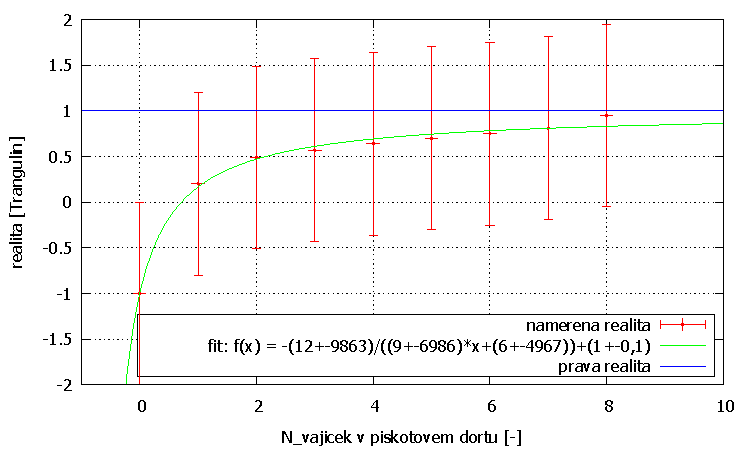
\includegraphics[width=\linewidth]{./att/vajicka.pdf}
	    	\caption{Závislost reality na kvalitě piškotového dortu. Vytvořeno ve $FUUPlot$.}
			\label{fig:g_2}
	\end{center}
	\end{figure}


Už Trangulin poukázal na to, že realita závisí na počtu použitých vajíček v dortu. Čím více vajíček, tím je realita přesnější. Zároveň pokud dort neobsahuje žádná vajíčka je možné vidět alternativní realitu, tu jsme objevili omylem při použití piškotového dortu PASCO Value. Domníváme se, že se Trangulinova žena nezbláznila, ale že vajíčka měla efekt červené pilulky a dostala se ven z Matrixu.
Jelikož nám naše realita nechtěla zkonvergovat, zamlčeli jsme chyby, fitli jsme ji (metodou nejlepších čtverců) a následně jsme chyby vykreslili do grafu. Lze vidět, že rovnice fitu je velmi přesná.

\subsubsection{Měření asistentů}

\begin{table}[h!]
\centering
\begin{tabular}{|l|r|r|r|r|r|r|}
 \hline
$asistent$&$Z$&$C$&$P$&$N$&$O$&$V$ \bigstrut\\ \hline
Péťa&-273,15&fit error&$\pm 95\ \mathrm{\%}$&over 9000&f(t)=-7t&100\bigstrut\\ \hline
Makki&$99,\overline{99}$&0&1,1&-&0&$9/10\cdot$Péťa\bigstrut\\ \hline
Otík&nedostatek dat&-&$\sqrt{-1}$&-&0&$\sqrt{-1}$\bigstrut\\ \hline
Míša&18&&&-&0&\bigstrut\\ \hline
Olinka&-&-&120&-&0&74,2\bigstrut\\ \hline
Tomík&100&-&50:50&-&0&99\bigstrut\\ \hline
\end{tabular}
\caption{Naměřené hodnoty pro jednotlivé asistenty: $Z$ je koeficient zábavnosti, $C$ koeficient čitelnosti hodnocení protokolu, $P$ koeficient přítomnosti u úlohy (u některých asistentů se ukázal být jen imaginární), $N$ faktor fyzického násilí, $O$ součinitel celkové jednotnosti oprav (v porovnání s ostatními asistenty) a $V$ faktor výslechu. Relativní chyby jednotlivých koeficientů jsme odhadli jako $\pm 1000\ \mathrm{\%}$  z důvodu velké závislosti na čase, náladě a celkovém stavu jednotlivých asistentů a studentů.}
\label{tabulka}
\end{table}

\subsection{Diskuse}

\subsubsection{Úloha pravdy}
Námi naměřené hodnoty se blíží těm na wikipedii, které jsme prohlásili za tabulkové a aniž bychom kdy měli v ruce citovaný zdroj, určitě tam bude hodnota stejná. Velikost chyby může být způsobena rozbitým přístrojem, měřili jsme totiž po velmi šikovné skupině. Pokud jsme ale přístroj omylem rozbili my, tak to na ně stejně svedeme. 

\subsubsection{Součinitel opruzu}
Měření součinitele opruzu se nakonec ukázalo být takový neuvěřitelný opruz, že jsme ho radši nezměřili. Měření stejně prohlašujeme za úspěšné, jelikož jsme se vyhnuli opruzu a to je úspěch vždycky.

\subsubsection{Měření asistentů}
Po napojení asistentů na elektrický obvod bylo vidět jejich nadšené klepání a cukání. Bohužel experiment odmítli opakovat, proto jsme jej měřili pouze jednou. Chyby při zapojování obvodu byly určitě způsobené nefunkčními kabely.

Nepodařilo se nám změřit všechny hodnoty u všech asistentů z důvodu časové tísně (naší, jejich i vrátné) a nedostatku alkoholu. Měření bychom zpřesnili použitím více asistentů a opakovaným měřením. Bohužel téměř žádný z experimentátorů se nehlásil na měření faktoru fyzického násilí.
\section{Závěr}
Z námi naměřených hodnot jsme došli k rozličným závěrům:

{\color{rarek}Rarek}: Napíšu to za chvíli…(takže 5 min před odevzdáním).

{\color{kuba}Kuba}: Jelikož jsme se zamotali ve schématu na Obr. \ref{fig:o_2}, jsme rádi, že nic neshořelo a i přes úspěšné zfixlování půlky hodnot nám experiment s překvapením vyšel.

{\color{tonda}Tonda}: Bohužel se nám nepodařilo naměřit všechna data a nemůžeme tak vyvodit dostatek pravdivých závěrů. Veškeré přiznané chyby měření jsou popsány v diskuzi. Nevylučuji ani možnost špatné interpretace dat.

{\color{dafit}daFit}: Měření bychom mohli prohlásit za úspěšné. Hodnoty koeficientů u jednotlivých asistentů se rozhodně blíží hodnotám z široce uznávaných Vymyšlených tabulek \cite{bib:vymyslene_tabulky}. 

{\color{pheter}Pheter}: Na základe nami nameraných hodnôt bolo potvrdené čo sa nepodarilo vyvrátiť. Avšak nedostatok latinského textu spôsobil rozvrátenie časopriestoru a teda sa našťastie, alebo aj na nešťastie biele na čiernom ukázalo neukázané.

{\color{andras}András}: A mérés volt teljesen hibátlan és viszonylag pontosan tükrözi faky minden, ami szükséges tudni a Praktikum. Hiba keletkezett, amikor mer okozta figyelmetlenség asszisztensek.

{\color{rarek}V\color{kuba}š\color{tonda}i\color{dafit}ch\color{pheter}n\color{andras}i}: 
Shodli jsme se, že zajímavou úlohou ke změření by bylo porovnání pěveckých schopností asistentů s těmi našimi při zpěvu přiložené písně \cite{bib:sound} a že měření koeficientu zábavnosti $Z$ by se dalo někdy dokončit a značně vylepšit, zvláště pak v neformálním prostředí zařízení sloužícího ke konzumaci fermentovaných ovocných nápojů a snižování mentální kompetence konzumentů.

\section{Použitá literatura}
\begin{thebibliography}{9}
\bibitem{bib:galaxy} Adams, D.: \textit{Stopařův průvodce Galaxií}, vyd. Ursa Minor:  Megadodo Publications, 3986 GY  ABB, \\ISBN: 4242424242
\bibitem{bib:ipsum} Cicero, M.T..: \textit{ De finibus bonorum et malorum}, vyd. Otrocké vydavateľstvo, C-L BC, \\ISBN: MDICXLIIX 
\bibitem{bib:magyar} Page, L., Brin, S. : \textit{Google Translate}, online, cit. 13. 14. 2000
\newline http://translate.google.com/
\bibitem{bib:vymyslene_tabulky}Kolektiv autorů: \textit{Vymyšlené tabulky co mají vždy takový hodnoty co potřebuješ}, vyd. General world information, \\ISBN: 133713371337  
\bibitem{bib:pristroje} Kolektiv KF, \emph{Návody k přístrojům} online, cit. 13. 13. 2013 \newline http://praktikum.fjfi.cvut.cz/documents/chybynav/navody-o.pdf
\bibitem{bib:sound} Zcela anonymní kolektiv: \textit{The Twelve Weeks of Lab Work}, online, cit. 13. 13. 2013
\newline https://soundcloud.com/user938917601/the-twelve-weeks-of-lab-work
\bibitem{bib:noty} Zcela anonymní kolektiv: \textit{Noty pro The Twelve Weeks of Lab Work}, online, cit. 13. 13. 2013
\newline http://broukej.cz/a/pra/pra\_noty.pdf
\bibitem{bib:protokol} Zcela anonymní kolektiv: \textit{Tento protokol}, online, cit. 13. 13. 2013
\newline http://broukej.cz/a/pra/pra\_protokol.pdf
\end{thebibliography} 

\section{Přílohy}
\subsection{Domácí příprava}
S přihlédnutím k doposud výborným výsledkům a mužnému vzhledu naší skupiny, jsme se rozhodli za koeficient $\varphi$ zvolit číslo 1,00. Během měření totiž několikrát použijeme metodu odvedení pozornosti (viz. Teoretický úvod), výsledky navíc proložíme metodou nejlepších čtverců (kdy čtverec odchylky přenásobíme libovolným číslem takovým, abychom ověřili přesně tu závislost, která se nám hodí). Fit nebudeme počítat ručně, ale s pomocí programu FUUplot.
\subsection{Statistické zpracování dat}
Aritmetický průměr X počítáme podle vzorce
\begin{equation}\label{eq:ch1}
X = \sum\limits_{i=1}^{n} \frac{x_i}{n},
\end{equation}
kde $x_i$ jsou vybrané hodnoty tak, aby nám vyšel požadovaný průměr a n je počet těchto hodnot. Tuto metodu nazýváme také Vyloučení (hrubých) chyb.

Maximální odhad chyby $\sigma_X$ počítáme podle vzorce
\begin{equation}\label{eq:ch2}
\sigma_X = \pm X,
\end{equation}

případně podle vzorců

\begin{equation}\label{eq:ch3}
\sigma_X = + X, \qquad \sigma_X = - X,
\end{equation}
pokud jsme si jisti, že naše chyby byly pouze pozitivní, resp. pouze negativní.

Používáme-li ve výpočtu zázračný koeficient fixu $\varphi$ (viz. 2.2.3), změní se hodnota výsledku $V$ podle vzorce

\begin{equation}\label{eq:ch4}
V = \left(\varphi \cdot X + (\sigma_X - \varphi \cdot \sigma_X ) \right),
\end{equation}

tedy platí, že celková chyba měření se s přesnějším koeficientem $\varphi$ zmenšuje.


\clearpage
\subsection{Obrázky}

\begin{figure}[h!]
	\begin{center}
    	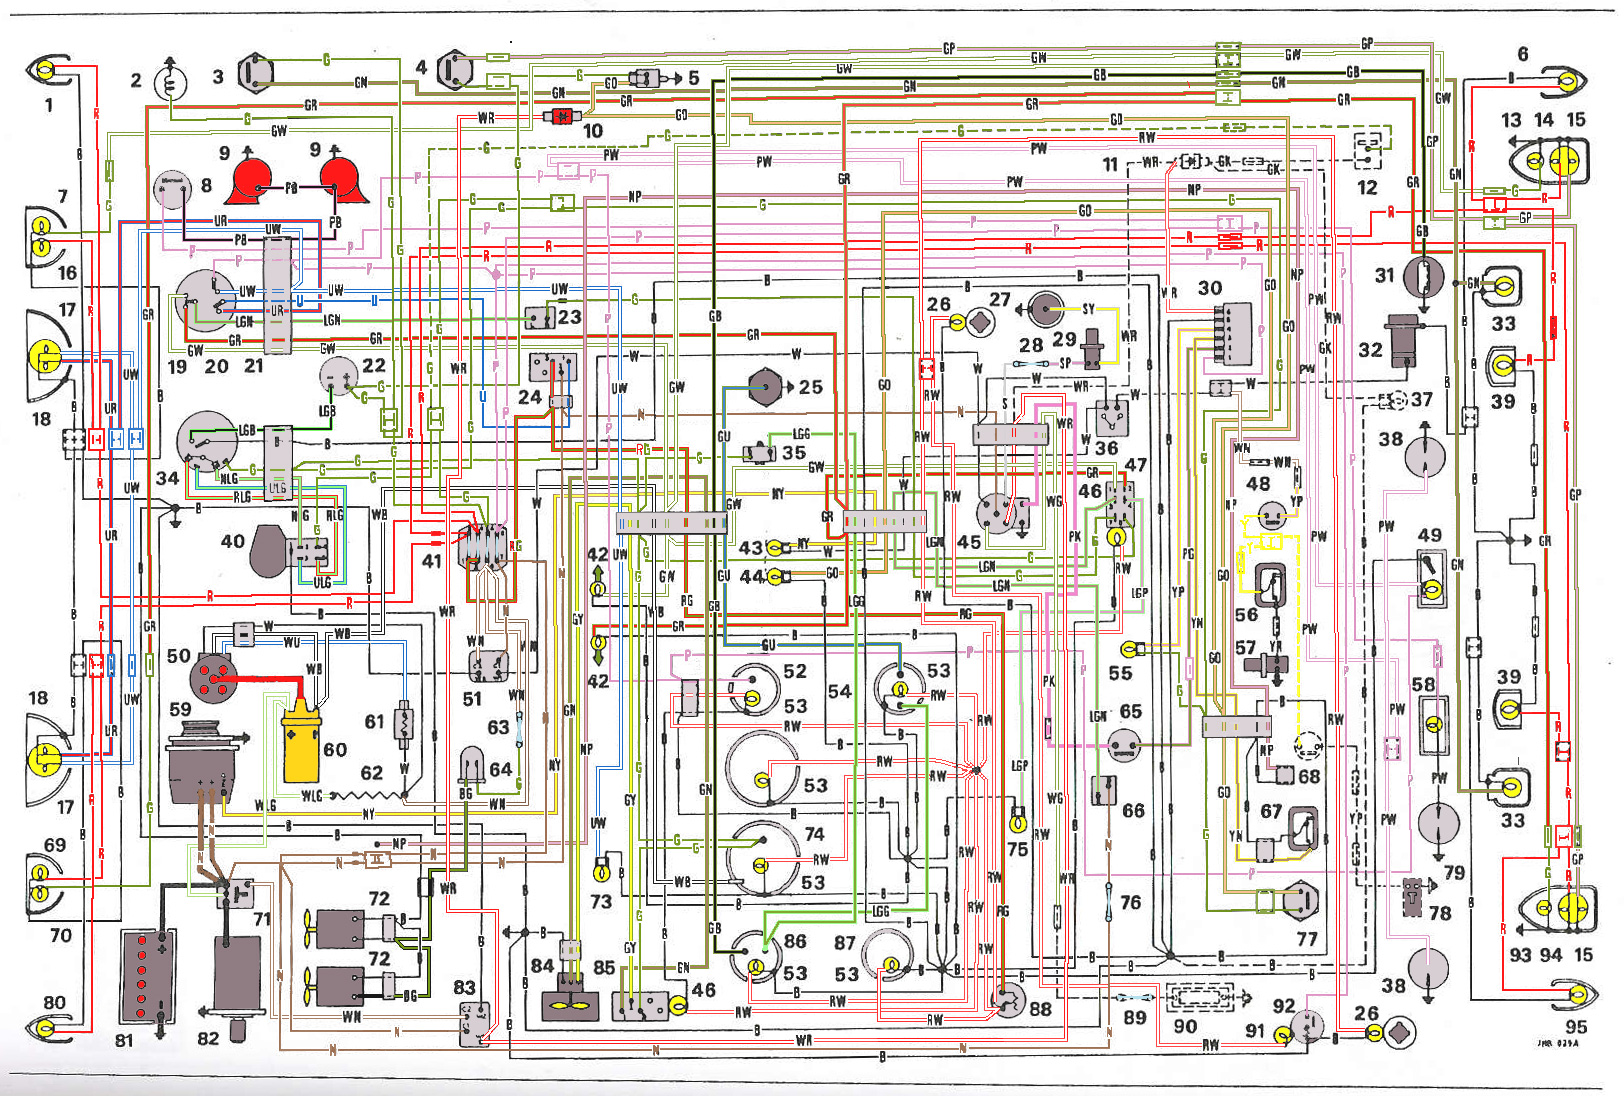
\includegraphics[width=0.7\linewidth]{./att/obvod.jpg}
        	\caption{Schéma zapojení 19 883 751 lízátek pomocného obvodu TESCO.  17 651 823. lízátko je kruciální. Převzato z \cite{bib:protokol}.}
        	\label{fig:g_3}
	\end{center}
	\end{figure}
	
			\begin{figure}[h!]
			\begin{center}
			    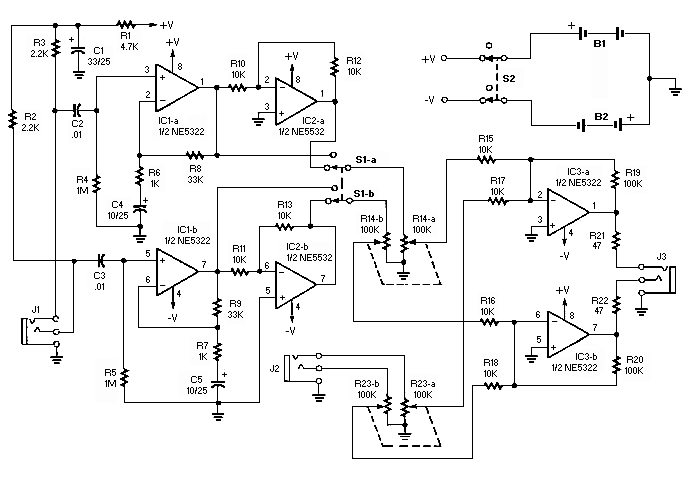
\includegraphics[width=0.6\linewidth]{./att/obvod.png}
			    	\caption{Vnitřní schéma měřící jednotky TESCO - je z něj okamžitě jasné, kam se co zapojuje a proč. Převzato z \cite{bib:protokol}.}
					\label{fig:o_2}
			\end{center}
			\end{figure}

	\begin{figure}[h!]
	\begin{center}
	    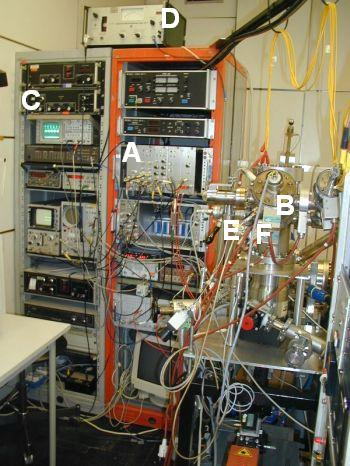
\includegraphics[width=0.45\linewidth]{./att/aparatura.jpg}
	    	\caption{Zapojení měřící aparatury: A je měřící jednotka TESCO - zapojení proveďte přesně podle obrázku, B nádoba na měření, C osciloskop, D voltmetr s rozsahem 0,005 V, E zapojení kabelů do nádoby a F matice nutná ke kalibraci přístroje. Na místě je teď novější verze přístroje, zapojení je ale velmi podobné. Převzato z \cite{bib:protokol}.}
			\label{fig:o_1}
	\end{center}
	\end{figure}
	


		\begin{figure}[h!]
		\begin{center}
		    
\includegraphics[width=0.2\linewidth]{./att/qrcode.png}
		    	\caption{QR kód vedoucí na hudební výsledek úlohy 1 \cite{bib:sound}.}
				\label{fig:qr}
		\end{center}
		\end{figure}





% --- Konec dokumentu --------------------------------------------------


\end{document}







